\documentclass{beamer}

\usepackage{amsmath}
\usepackage{graphicx}

\usetheme{AnnArbor}
\usecolortheme{crane}
\usefonttheme[onlymath]{serif}

\title{Deep Learning - Foundations and Concepts}
\subtitle{Chapter 3. Standard Distributions}
\author{nonlineark@github}
\date{\today}

\begin{document}

\begin{frame}
    \titlepage
\end{frame}

\begin{frame}
    \frametitle{Outline}
    \tableofcontents
\end{frame}

\section{Discrete Variables}

\begin{frame}
    \frametitle{Bernoulli distribution}
    \begin{itemize}
        \item Consider a binary random variable $x\in\{0,1\}$ and a parameter $0\le\mu\le{}1$, such that $p(x=1)=\mu$ and $p(x=0)=1-\mu$.
        \item Probability distribution: $\mathrm{Bern}(x;\mu)=\mu^{x}(1-\mu)^{1-x}$.
        \item Expectation: $E(x)=\mu$.
        \item Variance: $\mathrm{var}(x)=\mu(1-\mu)$.
    \end{itemize}
\end{frame}

\begin{frame}
    \frametitle{Bernoulli distribution}
    Model the Bernoulli distribution given observations $\{x_{1},\hdots,x_{N}\}$.
    \begin{align*}
        p(x_{1},\hdots,x_{N};\mu)&=\prod_{n=1}^{N}\mu^{x_{n}}(1-\mu)^{1-x_{n}} \\
        \log{}p(x_{1},\hdots,x_{N};\mu)&=\sum_{n=1}^{N}(x_{n}\log\mu+(1-x_{n})\log(1-\mu)) \\
        &=\log\mu\sum_{n=1}^{N}x_{n}+\log(1-\mu)(N-\sum_{n=1}^{N}x_{n}) \\
        \mu_{ML}&=\frac{1}{N}\sum_{n=1}^{N}x_{n}
    \end{align*}
\end{frame}

\begin{frame}
    \frametitle{Binomial distribution}
    \begin{itemize}
        \item Consider a random variable $m=\sum_{n=1}^{N}x_{n}$, where $x_{n}$ are independent random variables obey Bernoulli distribution with parameter $\mu$.
        \item Probability distribution: $\mathrm{Bin}(m;N,\mu)={N\choose{}m}\mu^{m}(1-\mu)^{N-m}$.
        \item Expectation: $E(m)=N\mu$.
        \item Variance: $\mathrm{var}(m)=N\mu(1-\mu)$.
    \end{itemize}
\end{frame}

\begin{frame}
    \frametitle{Multinomial distribution}
    \begin{itemize}
        \item Consider a random variable $x\in\{\mathrm{e}_{1},\hdots,\mathrm{e}_{K}\}$ and a parameter $\mu\in\mathbb{R}^{K}$, such that $p(x=\mathrm{e}_{k})=\mu_{k}$.
        \item Probability distribution: $p(x;\mu)=\prod_{k=1}^{K}\mu_{k}^{x_{k}}$.
        \item Expectation: $E(x)=\mu$.
        \item Covariance: $\mathrm{cov}(x)=\mathrm{diag}(\mu_{1},\hdots,\mu_{K})-\mu\mu^{T}$.
    \end{itemize}
\end{frame}

\begin{frame}
    \frametitle{Multinomial distribution}
    Model the generalized Bernoulli distribution given observations $x^{1},\hdots,x^{N}$.
    \begin{align*}
        p(x^{1},\hdots,x^{N};\mu)&=\prod_{n=1}^{N}\prod_{k=1}^{K}\mu_{k}^{x^{n}_{k}} \\
        \log{}p(x^{1},\hdots,x^{N};\mu)&=\sum_{n=1}^{N}\sum_{k=1}^{K}x^{n}_{k}\log\mu_{k}=\sum_{k=1}^{K}(\sum_{n=1}^{N}x^{n}_{k})\log\mu_{k} \\
        \mu_{ML}&=\frac{1}{N}\sum_{n=1}^{N}x^{n}
    \end{align*}
    For the last step, we used Lagrange multiplier to take into the constraint $\sum_{k=1}^{K}\mu_{k}=1$.
\end{frame}

\begin{frame}
    \frametitle{Multinomial distribution}
    \begin{itemize}
        \item Consider a random variable $m=\sum_{n=1}^{N}x^{n}$, where $x^{n}$ are independent random variables obey the generalized Bernoulli distribution with parameter $\mu$.
        \item Probability distribution: $\mathrm{Mult}(m;N,\mu)=\frac{N!}{\prod_{k=1}^{K}m_{k}!}\prod_{k=1}^{K}\mu_{k}^{m_{k}}$.
        \item Expectation: $E(m)=N\mu$.
        \item Covariance: $\mathrm{cov}(m)=N(\mathrm{diag}(\mu_{1},\hdots,\mu_{K})-\mu\mu^{T})$.
    \end{itemize}
\end{frame}

\section{The Multivariate Gaussian}

\begin{frame}
    \frametitle{Definition}
    For a single variable $x$, the Gaussian distribution can be written in the form:
    \begin{equation*}
        \mathcal{N}(x;\mu,\sigma^{2})=\frac{1}{\sqrt{2\pi\sigma^{2}}}\exp(-\frac{(x-\mu)^{2}}{2\sigma^{2}})
    \end{equation*}
    where $\mu$ is the mean and $\sigma^{2}$ is the variance. For a $D$-dimensional vector $x$, the multivariate Gaussian distribution takes the form:
    \begin{equation*}
        \mathcal{N}(x;\mu,\Sigma)=\frac{1}{(2\pi)^{\frac{D}{2}}(\det\Sigma)^{\frac{1}{2}}}\exp(-\frac{1}{2}(x-\mu)^{T}\Sigma^{-1}(x-\mu))
    \end{equation*}
    where $\mu$ is the $D$-dimensional mean vector, $\Sigma$ is the $D\times{}D$ covariance matrix.
\end{frame}

\begin{frame}
    \frametitle{Geometry of the Gaussian}
    Without loss of generality, we assume $\Sigma$ is symmetric. As a self-adjoint operator, there exists an orthonormal basis $(u_{1},\hdots,u_{D})$ under which $\Sigma$ is diagonalized:
    \begin{equation*}
        \mathrm{diag}(\lambda_{1},\hdots,\lambda_{D})=U^{T}\Sigma{}U
    \end{equation*}
    where $U$ is the orthogonal matrix whose $j$th column is $u_{j}$. Now let $x-\mu=Uy$, we see that under the new basis, the multivariate Gaussian takes the form:
    \begin{align*}
        \mathcal{N}(x;\mu,\Sigma)&=\frac{1}{(2\pi)^{\frac{D}{2}}(\lambda_{1}\hdots\lambda_{D})^{\frac{1}{2}}}\exp(-\frac{1}{2}y^{T}\mathrm{diag}^{-1}(\lambda_{1},\hdots,\lambda_{D})y)|\det{}U| \\
        &=\frac{1}{\sqrt{2\pi\lambda_{1}}\hdots\sqrt{2\pi\lambda_{D}}}\exp(-\frac{1}{2}\sum_{d=1}^{D}\frac{y_{d}^{2}}{\lambda_{d}}) \\
        &=\prod_{d=1}^{D}\frac{1}{\sqrt{2\pi\lambda_{d}}}\exp(-\frac{y_{d}^{2}}{2\lambda_{d}})
    \end{align*}
\end{frame}

\begin{frame}
    \frametitle{Geometry of the Gaussian}
    \begin{figure}
        \caption{Geometry of the Gaussian}
        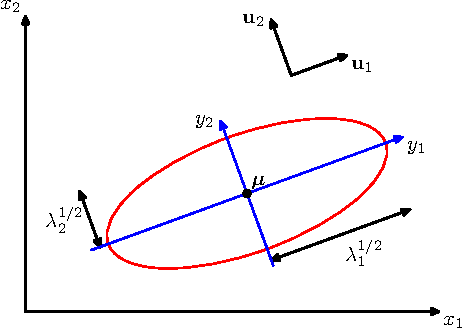
\includegraphics{Figure_3.pdf}
    \end{figure}
\end{frame}

\begin{frame}
    \frametitle{Geometry of the Gaussian}
    It's easy to see that the multivariate Gaussian is indeed normalized:
    \begin{align*}
        \int\mathcal{N}(x;\mu,\Sigma)\mathrm{d}x&=\int\prod_{d=1}^{D}\frac{1}{\sqrt{2\pi\lambda_{d}}}\exp(-\frac{y_{d}^{2}}{2\lambda_{d}})\mathrm{d}y \\
        &=\prod_{d=1}^{D}\int_{-\infty}^{+\infty}\frac{1}{\sqrt{2\pi\lambda_{d}}}\exp(-\frac{y_{d}^{2}}{2\lambda_{d}})\mathrm{d}y_{d} \\
        &=1
    \end{align*}
\end{frame}

\begin{frame}
    \frametitle{Expectation and covariance}
    Similarly, we can calculate the expectation and covariance of the multivariate Gaussian:
    \begin{align*}
        E(x)&=\int\mathcal{N}(x;\mu,\Sigma)x\mathrm{d}x \\
        &=\int\prod_{d=1}^{D}\frac{1}{\sqrt{2\pi\lambda_{d}}}\exp(-\frac{y_{d}^{2}}{2\lambda_{d}})(\mu+Uy)|\det{}U|\mathrm{d}y \\
        &=\mu+U\int\prod_{d=1}^{D}\frac{1}{\sqrt{2\pi\lambda_{d}}}\exp(-\frac{y_{d}^{2}}{2\lambda_{d}})y\mathrm{d}y \\
        &=\mu
    \end{align*}
\end{frame}

\begin{frame}
    \frametitle{Expectation and covariance}
    \begin{align*}
        E(xx^{T})&=\int\mathcal{N}(x;\mu,\Sigma)xx^{T}\mathrm{d}x \\
        &=\int\prod_{d=1}^{D}\frac{1}{\sqrt{2\pi\lambda_{d}}}\exp(-\frac{y_{d}^{2}}{2\lambda_{d}})(\mu+Uy)(\mu+Uy)^{T}|\det{}U|\mathrm{d}y \\
        &=\mu\mu^{T}+U(\int\prod_{d=1}^{D}\frac{1}{\sqrt{2\pi\lambda_{d}}}\exp(-\frac{y_{d}^{2}}{2\lambda_{d}})yy^{T}\mathrm{d}y)U^{T} \\
        &=\mu\mu^{T}+U\mathrm{diag}(\lambda_{1},\hdots,\lambda_{D})U^{T}=\mu\mu^{T}+\Sigma \\
        \mathrm{cov}(x)&=E(xx^{T})-E(x)E(x^{T})=\Sigma
    \end{align*}
\end{frame}

\begin{frame}
    \frametitle{The good and the bad about the Gaussian}
    \begin{itemize}
        \item The Gaussian distribution arises in many different contexts:
        \begin{itemize}
            \item The distribution that maximizes the entropy is the Gaussian.
            \item Central limit theorem.
        \end{itemize}
        \item The Gaussian distribution has many important analytical properties.
        \item For large $D$, the total number of parameters grows quadratically with $D$, manipulating and inverting the large matrices can become prohibitive.
        \item The Gaussian distribution is intrinsically unimodal, and so is unable to provide a good approximation to multimodal distributions.
    \end{itemize}
\end{frame}

\begin{frame}
    \frametitle{Conditional distribution and marginal distribution}
    \begin{block}{Problem}
        Suppose $x$ obeys the Gaussian distribution $\mathcal{N}(x;\mu,\Sigma)$. If we partition $x$ into $x_{a}$ and $x_{b}$, that is $x=\begin{pmatrix}
            x_{a} \\
            x_{b}
        \end{pmatrix}$, what is the expression for the conditional distribution $p(x_{a}|x_{b})$ and the marginal distribution $p(x_{a})$?
    \end{block}
\end{frame}

\begin{frame}
    \frametitle{Conditional distribution and marginal distribution}
    First step, let's also partition the mean and covariance accordingly:
    \begin{align*}
        \mu&=\begin{pmatrix}
            \mu_{a} \\
            \mu_{b}
        \end{pmatrix} \\
        \Sigma&=\begin{pmatrix}
            \Sigma_{aa}&\Sigma_{ab} \\
            \Sigma_{ba}&\Sigma_{bb}
        \end{pmatrix}
    \end{align*}
    Because $\Sigma^{-1}$ (called the precision matrix) appears frequently, we also partition $\Sigma^{-1}$:
    \begin{equation*}
        \Sigma^{-1}=\begin{pmatrix}
            \Lambda_{aa}&\Lambda_{ab} \\
            \Lambda_{ba}&\Lambda_{bb}
        \end{pmatrix}
    \end{equation*}
    Notice that because $\Sigma$ and $\Sigma^{-1}$ are symmetric, $\Sigma_{aa}$, $\Sigma_{bb}$, $\Lambda_{aa}$ and $\Lambda_{bb}$ are symmetric as well. Further, we have $\Sigma_{ba}=\Sigma_{ab}^{T}$ and $\Lambda_{ba}=\Lambda_{ab}^{T}$.
\end{frame}

\begin{frame}
    \frametitle{Conditional distribution and marginal distribution}
    Second step, let's complete the square! Notice:
    \begin{equation*}
        (x-\mu)^{T}\Sigma^{-1}(x-\mu)=x\Sigma^{-1}x-2x^{T}\Sigma^{-1}\mu+\mu^{T}\Sigma^{-1}\mu
    \end{equation*}
    For conditional distribution $p(x_{a}|x_{b})$:
    \begin{align*}
        (x-\mu)^{T}\Sigma^{-1}(x-\mu)&=\begin{pmatrix}
            x_{a}^{T}-\mu_{a}^{T}&x_{b}^{T}-\mu_{b}^{T}
        \end{pmatrix}
        \begin{pmatrix}
            \Lambda_{aa}&\Lambda_{ab} \\
            \Lambda_{ba}&\Lambda_{bb}
        \end{pmatrix}
        \begin{pmatrix}
            x_{a}-\mu_{a} \\
            x_{b}-\mu_{b}
        \end{pmatrix} \\
        &=x_{a}^{T}\Lambda_{aa}x_{a}-2x_{a}^{T}(\Lambda_{aa}\mu_{a}-\Lambda_{ab}(x_{b}-\mu_{b}))+\mathrm{const}
    \end{align*}
    Compare, we see:
    \begin{align*}
        \Sigma_{x_{a}|x_{b}}^{-1}&=\Lambda_{aa} \\
        \Sigma_{x_{a}|x_{b}}&=\Lambda_{aa}^{-1} \\
        \Sigma_{x_{a}|x_{b}}^{-1}\mu_{x_{a}|x_{b}}&=\Lambda_{aa}\mu_{a}-\Lambda_{ab}(x_{b}-\mu_{b}) \\
        \mu_{x_{a}|x_{b}}&=\mu_{a}-\Lambda_{aa}^{-1}\Lambda_{ab}(x_{b}-\mu_{b})
    \end{align*}
\end{frame}

\begin{frame}
    \frametitle{Conditional distribution and marginal distribution}
    For marginal distribution, $p(x_{a})=\int{}p(x_{a},x_{b})\mathrm{d}x_{b}$. Let's first complete the square for $x_{b}$ to integrate it out:
    \begin{align*}
        &(x-\mu)^{T}\Sigma^{-1}(x-\mu)=\begin{pmatrix}
            x_{a}^{T}-\mu_{a}^{T}&x_{b}^{T}-\mu_{b}^{T}
        \end{pmatrix}
        \begin{pmatrix}
            \Lambda_{aa}&\Lambda_{ab} \\
            \Lambda_{ba}&\Lambda_{bb}
        \end{pmatrix}
        \begin{pmatrix}
            x_{a}-\mu_{a} \\
            x_{b}-\mu_{b}
        \end{pmatrix} \\
        &=x_{b}^{T}\Lambda_{bb}x_{b}-2x_{b}^{T}\Lambda_{bb}(\mu_{b}-\Lambda_{bb}^{-1}\Lambda_{ba}(x_{a}-\mu_{a}))+\cdots \\
        &=x_{b}^{T}\Lambda_{bb}x_{b}-2x_{b}^{T}\Lambda_{bb}m+m^{T}\Lambda_{bb}m+\cdots \\
        &=(x_{b}-m)^{T}\Lambda_{bb}(x_{b}-m)+\cdots
    \end{align*}
    where $m=\mu_{b}-\Lambda_{bb}^{-1}\Lambda_{ba}(x_{a}-\mu_{a})$. We see that when integrating $x_{b}$, the result will be a constant not depending on $x_{a}$, although $m$ depends on $x_{a}$.
\end{frame}

\begin{frame}
    \frametitle{Conditional distribution and marginal distribution}
    Which means, we can take a look at the terms left in $\cdots$, and complete the square for $x_{a}$ to get the mean and the covariance for $x_{a}$:
    \begin{equation*}
        \cdots=(x_{a}-\mu_{a})^{T}(\Lambda_{aa}-\Lambda_{ab}\Lambda_{bb}^{-1}\Lambda_{ba})(x_{a}-\mu_{a})
    \end{equation*}
    We see that:
    \begin{align*}
        \Sigma_{x_{a}}&=(\Lambda_{aa}-\Lambda_{ab}\Lambda_{bb}^{-1}\Lambda_{ba})^{-1} \\
        \mu_{x_{a}}&=\mu_{a}
    \end{align*}
    Through a rather ugly equation (known as Schur complement), we can simplify the expression for $\Sigma_{x_{a}}$ to a much nicer one:
    \begin{equation*}
        \Sigma_{x_{a}}=\Sigma_{aa}
    \end{equation*}
\end{frame}

\begin{frame}
    \frametitle{Conditional distribution and marginal distribution}
    \begin{figure}
        \caption{The marginal distribution and the conditional distribution}
        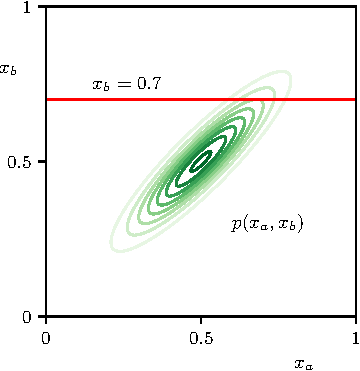
\includegraphics[width=0.4\textwidth]{Figure_5_a.pdf}
        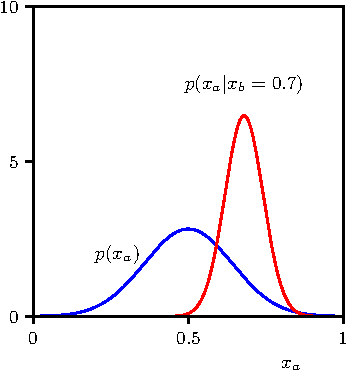
\includegraphics[width=0.4\textwidth]{Figure_5_b.pdf}
    \end{figure}
\end{frame}

\end{document}